\documentclass[a4paper,12pt]{article} % тип документа

% report, book

% Рисунки
\usepackage{graphicx}
\usepackage{wrapfig}

\usepackage{hyperref}
\usepackage[rgb]{xcolor}
\hypersetup{				% Гиперссылки
    colorlinks=true,       	% false: ссылки в рамках
	urlcolor=blue          % на URL
}

%  Русский язык

\usepackage[T2A]{fontenc}			% кодировка
\usepackage[utf8]{inputenc}			% кодировка исходного текста
\usepackage[english,russian]{babel}	% локализация и переносы


% Математика
\usepackage{amsmath,amsfonts,amssymb,amsthm,mathtools} 


\usepackage{wasysym}

\author{Анна Назарчук Б02-109}
\title{1.1.1 Определение систематических и случайных погрешностей при измерении удельного сопротивления нихромовой проволоки}
\date{}
\begin{document}
\maketitle

\section{Аннотация}
В работе сопротивление нихромовой проволоки измеряется несколькимим методами: с помощью амперметра и вольтметра, классическим методом моста постоянного тока (мост Уитстона). Размеры проволоки получаются с использованием линейки, микрометра, штангенциркуля. Исследуются систематические и случайные ошибки измерений.

\section{Теоретические сведения}
Удельное споротивление однородной по материалу и толщине проволоки круглого сечения может быть определено по формуле \ref{удсоп}:
\begin{equation}\label{удсоп}
\rho=\frac{R_{\text{пр}}}{l}\frac{\pi d_{\text{ср}}^2}{4}
\end{equation}
где $R_{\text{пр}}$ - сопротивление измеряемого отрезка проволоки, $l$ - его длина, $d_{\text{ср}}$ - средний диаметр проволоки.

Величину $R_{\text{пр}}$ измерим с помощью одной из схем, представленных на рис. \ref{схемы}
\begin{figure}[h!]
\begin{center}
\includegraphics[width=0.9\textwidth]{схемы}
\end{center}
\caption{Схемы для измерения сопротивления при помощи амперметра и вольтметра} \label{схемы}
\end{figure}
Для случая а) вольтметр измеряет напряжение ($U_a$) на концах проволоки, а амперметр измеряет не ток, идущий через проволоку, а сумму токов ($I_a$), проходящих через проволоку и вольтметр . Поэтому 
\begin{equation}\label{рпр1}
R_{\text{пр1}}=\frac{U_a}{I_a}=R_{\text{пр}} \frac{R_V}{R_V+R_{\text{пр}}}
\end{equation}
Откуда для схемы а):
\begin{equation}\label{ра}
R_{\text{пр}}=R_{пр1} \frac{R_V}{R_V-R_{\text{пр1}}}=R_{\text{пр1}} \frac{R_{\text{пр1}}}{1-\frac{R_{\text{пр1}}}{R_V}}\approx R_{\text{пр1}} \left( 1+\frac{R_{\text{пр1}}}{R_V}\right)
\end{equation}
Для случая б) амперметр измеряет силу тока ($I_\text{б}$) через проволоку, вольтметр измеряет напряжение не на концах проволоки, а напряжение ($U_\text{б}$) на амперметре и проволоке. Поэтому
\begin{equation}\label{рпр2}
R_{\text{пр2}}=\frac{U_\text{б}}{I_\text{б}}=R_{\text{пр}}+R_A
\end{equation}
Откуда для схемы б):
\begin{equation}\label{рб}
R_{\text{пр}}=R_{\text{пр2}} \left( 1-\frac{R_{\text{А}}}{R_{\text{пр2}}} \right)
\end{equation}
Более точным методом измерения сопротивления является метод моста постоянного тока (мост Уитстона).

\section{Оборудование}
\textbf{Линейка} : $\Delta_{\text{лин}} = \pm 0.5$ мм (по цене деления). 

\textbf{Штангенциркуль}: $\Delta_{\text{шт}} = \pm 0.05$ мм (маркировка производителя)

\textbf{Микрометр} : $\Delta_{\text{мкм}} = \pm 0.01$ мм (маркировка производителя)

\begin{table}
\caption{Характеристики вольтметра}
\begin{tabular}{|c|c|}
\hline 
Система & Магнитно-электрическая \\ 
\hline 
Класс точности & 0.5 \\ 
\hline 
Шкала & линейная, 150 делений  \\ 
\hline 
Предел измерений & 0.75 В \\ 
\hline 
Цена деления & 5 мВ \\ 
\hline 
Внутреннее сопротивление & 250 Ом \\ 
\hline 
Погрешность при считывании со шкалы & $\pm 2.5$ мВ \\ 
\hline 
Макс. погрешность & $\pm3.75$ мВ \\ 
\hline 
\end{tabular} 
\end{table}

\begin{table}
\caption{Характеристики амперметра}
\begin{tabular}{|c|c|}
\hline 
Система & Цифровая \\  
\hline 
Разрядность дисплея & 5 ед. \\ 
\hline 
Внутреннее сопротивление & 1,2 Ом \\ 
\hline 
Погрешность & $\pm (0.002X+0.02)$ мА \\ 
\hline 
\end{tabular} 
\end{table}
Исходя из характеристик приборов можно заметить, что при $R_{\text{пр}} \approx 5$ Ом
\[\frac{R_{\text{А}}}{R_{\text{пр2}}} > \frac{R_{\text{пр1}}}{R_V}\]
Поэтому измерения будем проводить с помощью схемы 1а.

\begin{table}
\caption{Характеристики моста постоянного тока P4833}
\begin{tabular}{|c|c|}
\hline 
Класс точности & 0.1 \\ 
\hline 
Разрядность магазина сопротивлений & 5 ед. \\ 
\hline 
Используемый диапазон измерений & $10^{-4} - 10$ Ом \\ 
\hline 
Погрешность в данном диапазоне & $\pm 0.01$ Ом \\  
\hline 
\end{tabular} 
\end{table}

\section{Результаты измерений и обработка данных}
\subsection{Измерение диаметра проволоки}
Измерения проводились штангенциркулем и микрометром многократно на разных участках проволоки. Результаты представлены в таблице \ref{Диаметр}. Обработанные данные можно найти в таблице \ref{Диаметробр}.
\begin{table}
\label{Диаметр}
\caption{Результаты измерения диаметра проволоки}
\begin{tabular}{|c|c|c|c|c|c|c|c|c|c|c|}
\hline 
$N_{\text{изм}}$ & 1 & 2 & 3 & 4 & 5 & 6 & 7 & 8 & 9 & 10 \\ 
\hline 
Микрометр: d, мм & 0.36 & 0.36 & 0.35 & 0.36 & 0.36 & 0.36 & 0.36 & 0.36 & 0.36 & 0.35 \\ 
\hline 
Штангенциркуль: d, мм & 0.35 & 0.35 & 0.35 & 0.35 & 0.35 & 0.35 & 0.35 & 0.35 & 0.35 & 0.35 \\ 
\hline 
\end{tabular} 
\end{table}

\begin{table}
\caption{Обработка результатов измерения диаметра}
\label{Диаметробр}
\begin{tabular}{|c|c|c|}
\hline 
 & Микрометр & Штангенциркуль \\ 
\hline 
Средний диаметр: $\overline{d}=\frac{\sum d_i}{N}$ & 0.358 & 0.35 \\ 
\hline 
Стандартное отклонение: $\sigma_d=\sqrt{\frac{1}{N-1}\sum (d_i-\overline{d})^2}$ & 0.004&0 \\ 
\hline 
Случайная погрешность среднего: $\sigma_{\overline{d}}=\frac{\sigma_d}{\sqrt{N}}$ & 0.001 & 0 \\ 
\hline 
Инструментальная погрешность: $\Delta$ & 0.01 & 0.05 \\ 
\hline 
Полная погрешность: $\sigma_{\text{пол}}=\sqrt{\sigma_{\overline{d}}^2+\sigma_d^2}$ & 0.01 & 0.05 \\ 
\hline 
Окончательные результаты измерения:  & 0.358 $\pm$ 0.01 & 0.35 $\pm$ 0.05 \\
\hline 
\end{tabular} 
\end{table}

\subsection{Измерения сопротивления проволоки}
Результаты измерений напряжения и силы тока в зависимости от длины исследуемого образца проволоки представлены в таблице \ref{ампвол} и на графике (рис. \ref{графики})
\begin{table}
\caption{Результаты измерения напряжения и силы тока}
\begin{tabular}{|c|c|c|c|c|c|}
\hline 
   \multicolumn{6}{|c|}{$l = 50 \pm 0.05$ см} \\ 
\hline 
$I_a$, мА & 66.34 & 75.67 & 88.57 & 103.58 & 120.84 \\ 
\hline 
$V_a$, деления & 66 & 75 & 88 & 103 & 120 \\ 
\hline 
$V_a$, мВ & 330 & 375 & 440 & 515 & 600  \\ 
\hline 

$I_a$, мА & 143.53 & 148.69 & 129.59 & 105.21 & 96.79  \\ 
\hline 
$V_a$, деления & 143 & 148 & 129 & 105 & 96 \\ 
\hline 
$V_a$, мВ & 715 & 740 & 645 & 525 & 480 \\ 
\hline 
\hline

   \multicolumn{6}{|c|}{$l = 30 \pm 0.05$ см} \\ 
\hline 
$I_a$, мА &151.06 & 179.84 & 237.59 & 142.59 & 225.72 \\ 
\hline 
$V_a$, деления & 92 & 110 & 145 & 87 & 138 \\ 
\hline 
$V_a$, мВ & 460 & 550 & 725 & 435 & 690 \\ 
\hline 

$I_a$, мА & 143.92 & 191.53 & 198.91 & 181.2 & 169.85  \\ 
\hline 
$V_a$, деления & 88 & 117 & 121 & 111 & 104 \\ 
\hline 
$V_a$, мВ & 440 & 585 & 605 & 555 & 520 \\ 
\hline 
\hline 

   \multicolumn{6}{|c|}{$l = 20 \pm 0.05$ см} \\ 
\hline 
$I_a$, мА & 261.51 & 351.76 & 269.82 & 201.19 & 257.51  \\ 
\hline 
$V_a$, деления & 109 & 147 & 113 & 84 & 107 \\ 
\hline 
$V_a$, мВ & 545 & 735 & 565 & 420 & 535 \\ 
\hline 

$I_a$, мА & 329.57 & 297.29 & 347.21 & 242.69 & 215.57 \\ 
\hline 
$V_a$, деления & 138 & 124 & 145 & 101 & 90 \\ 
\hline 
$V_a$, мВ & 690 & 620 & 725 & 505 & 450  \\ 
\hline 

\end{tabular} 
\label{ампвол}
\end{table}

\begin{figure}[h!]
\begin{center}
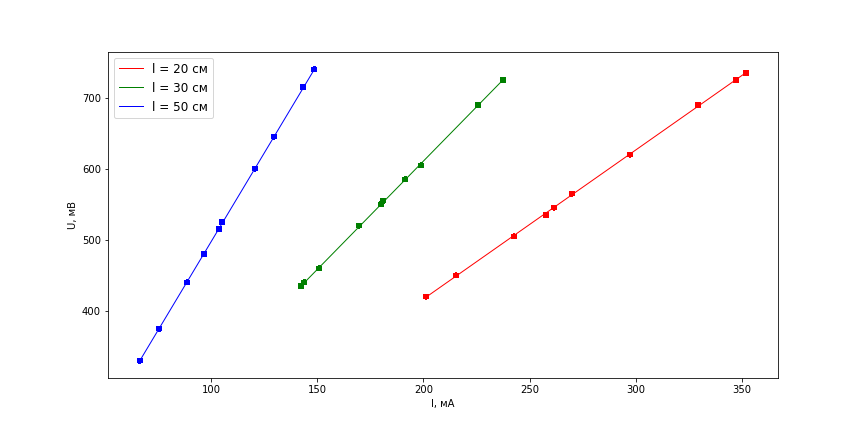
\includegraphics[width=\textwidth]{графики}
\end{center}
\caption{Результаты измерений напряжения $V$ (мВ) в зависимости от тока $I$ (мА) для проволок разной длины $l$ и их линейная аппроксимация } 
\label{графики}
\end{figure}

Для каждой длины $ l $ проводим расчет $R_{\text{ср}}$ методом наименьших квадратов для прямой, проходящей через начало координат (используется Python). Найдем случайную ошибку измерения по формуле:
\begin{equation}
\sigma_{R_{\text{ср}}}^{\text{случ}}=\frac{1}{\sqrt{10}}\sqrt{\frac{\langle V^2 \rangle}{\langle I^2 \rangle}-R_{\text{ср}}^2}
\end{equation}
Систематическую погрешность $R_{\text{ср}}$ оценим по формуле:
\begin{equation}
\frac{\sigma_{R_{\text{ср}}}^{\text{случ}}}{R_{\text{ср}}}=\sqrt{\left( \frac{\sigma_V}{V} \right)^2+\left( \frac{\sigma_I}{I} \right)^2}
\end{equation}
Результаты измерения сопротивления проволок с помощью вольтметра и амперметра, а также используя мост Уинстона с учетом погрешностей представлены в таблице \ref{сопротив}. Помимо этого учитывается поправка в измерении сопротивления проволоки по формуле \ref{ра}
\begin{table}

\caption{Результаты измерения сопротивления проволок}
\begin{tabular}{|c|c|c|c|c|c|c|}
\hline 
$l, $см & $R_{\text{ср}}$, Ом & $\sigma_{R_{\text{ср}}}^{\text{случ}}$, Ом & $\sigma_{R_{\text{ср}}}^{\text{сист}}$, Ом & $\sigma_{R_{\text{ср}}}$, Ом & $R_{\text{пр}}$, Ом & $R_0$, Ом \\ 
\hline 
20 & 2.09 & 0.001 & 0.012 & 0.012 & 2.12$\pm$ 0.012& 2.23 $\pm$ 0.01 \\ 
\hline 
30 & 3.05 & 0.002 & 0.017 & 0.017 & 3.09$\pm$  0.017& 3.32 $\pm$ 0.01 \\ 
\hline 
50 & 4.99 & 0.003 & 0.027 & 0.028 & 5.09$\pm$ 0.028& 5.35 $\pm$ 0.01 \\ 
\hline 
\end{tabular} 
\label{сопротив}
\end{table} 
Можно заметить, что случайная погрешность измерения сопротивления мала, все ошибки происходят из-за систематических ошибок приборов: амперметра и вольтметра. Результаты измерения практически равняются результатам контрольных измерений при помощи моста Уинстона.
\subsection{Измерение удельного сопротивления проволоки}
Определим площадь поперечного сечения проволоки с учетом погрешности, используя данные для диаметра $d$ и $\sigma_d$ из измерений микрометром:
\begin{equation}
S = \frac{\pi d^2}{4}=0.1\cdot10^{-6}  \text{м}^2
\end{equation}
\begin{equation}
\sigma_S=2\frac{\sigma_d}{d}S=5.6\cdot10^{-9} \text{м}^2
\end{equation}

Найдем удельное сопротивление проволоки по формуле:
\begin{equation}
\rho = R\frac{S}{l}
\end{equation}
\begin{equation}
\sigma_{\rho} = \sqrt{\left( \frac{\sigma_R}{R} \right)^2+\left( \frac{\sigma_d}{d} \right)^2+\left(2 \frac{\sigma_l}{l} \right)^2}
\end{equation}
Результаты для каждой из длин представлены в таблице \ref{удсопрот}

\begin{table}
\caption{Результаты измерения $\rho$ для каждой из длин проволок}
\begin{tabular}{|c|c|c|}
\hline 
$l$, см & $\rho$, $10^{-6}$ Ом $\cdot$м &$\sigma_{\rho}$, $10^{-8}$Ом$\cdot$м \\ 
\hline 
20 & 1.06 & 5.96 \\ 
\hline 
30 & 1.03 & 5.78 \\ 
\hline 
50 & 1.02 & 5.73 \\ 
\hline 
\end{tabular} 
\label{удсопрот}
\end{table}
Окончательно $\rho = (1.04 \pm 0.06)\cdot 10^{-6}$ Ом$\cdot$м.
\section{Вывод}
Полученное значение $\rho$ сравним с табличными данными. Согласно справочнику (Физические величины. М.: Энергоиздат, 1991.) для удельного сопротивления нихрома при $20^{\circ}C$ наиболее близкое значение к получившемуся в работе для сплава: 70-80\% Ni, 20 \% Cr, 0-2\% Mn (проценты по массе).

Использованный в работе метод измерения позволяет получать значения $R$ с достаточно низкой погрешностью ($\backsim 0.5 \%$). Основной вклад в погрешность $\rho$ ($\backsim 6 \%$) вносит погрешность измерения диаметра ($\backsim 3 \%$). Однако систематическая погрешность измерения диаметра существенно больше случайной ее составляющей, поэтому улучшить измерения при проведении большего числа измерений теми же приборами не получится, как и не получится узнать про однородность проволоки по диаметру. Только измерения на более качественном и точном оборудовании могут привести к уменьшению погршености измерения.
\end{document}